\section{Supplementary Simulation Results for Adaptive Experiments}\label{sec:additional-simulation-sequential}

\subsection{Finite Sample Properties of Lemma \ref{lemma:asymptotic-tau-sigma}}\label{subsec:finite-sample-lemma}

We verify the finite sample properties of Lemma \ref{lemma:asymptotic-tau-sigma} using simulated data. The simulated data with $N$ units and $T$ time periods is generated as follows 
\[Y_{is} = \alpha_i + \beta_s + \tau_0 z_{is} + \varepsilon_{is},\]
where 
\[\alpha_i \stackrel{\iid}{\sim} \mathcal{N}(0,1), \qquad \beta_s \stackrel{\iid}{\sim} \mathcal{N}(0,1), \qquad \varepsilon_{is} \stackrel{\iid}{\sim} \mathcal{N}(0,\sigma^2_\varepsilon),  \]
and $Z = [z_{is}]_{i\in[N],s\in [T]}$ is randomly sampled from the treatment designs that satisfy $N^{-1} \sum_{i} z_{is} = {(2s - 1 - T)}/{T}$ ({\it i.e.}, the optimal design with instantaneous effect only). In this case, all $N$ units are NTU. 

Let $\hat{\tau}$ be the \within estimator of $\hat{\tau}_0$ and let $\estsigmasq$ be the estimated $\sigma_\varepsilon^2$ using the formula \eqref{eqn:second-moment-sigma-estimator}. We report the standardized $\hat{\tau}$, that is, 
\[ \hat{\tau}_{\mathsf{ss}} =  \sqrt{N} \cdot \frac{\hat{\tau} - \tau_0}{[\estsigmasq /(T \cdot \funfrac(\bm{\omega}_{\fcs, 1:T}, T))]^{1/2}} \]
and the standardized $\estsigmasq$, that is, \[\estsigmasq_{\mathsf{ss}} =  \sqrt{N} \cdot \frac{\estsigmasq - \sigma^2}{[\estxidaggersq/T]^{1/2}} \]
where $\estxidaggersq = \estxisq + {2}/{(T-1)} \cdot (\estsigmasq)^2$ and $\estxisq$ is estimated using the formula \eqref{eqn:fourth-moment-sigma-estimator}. 

We also report the standardized $\estsigmasq$ by a naive plug-in estimator of the variance of $\estsigmasq$, that is, 
\[\estsigmasq_{\mathsf{ss},\mathrm{naive}} =  \sqrt{N} \cdot \frac{\estsigmasq - \sigma^2}{[\estxisq_{\mathrm{naive}}/T]^{1/2}}, \]
where 
\[\estxisq_{\mathrm{naive}} = \frac{1}{NT} \sum_{i,s} \left( (\dot{y}_{is} - \hat{\tau} \cdot \dot{z}_{is})^2 - \estsigmasq \right)^2. \]

We repeat the above data generating and estimation procedure for 1,000 times and report the histograms of $\hat{\tau}_{\mathsf{ss}}$, $\estsigmasq_{\mathsf{ss}}$, and $\estsigmasq_{\mathsf{ss},\mathrm{naive}}$ in Figure \ref{fig:test-asymptotics} for various $T$.  As shown in Figure \ref{fig:test-asymptotics}, the histograms of $\hat{\tau}_{\mathsf{ss}}$ and  $\estsigmasq_{\mathsf{ss}}$ are close to the standard normal density function, showing the good finite sample properties of $\hat{\tau}_{\mathsf{ss}}$ and  $\estsigmasq_{\mathsf{ss}}$. However, the histograms of $\estsigmasq_{\mathsf{ss},\mathrm{naive}} $ deviate from the standard normal density function and the deviation is larger for a smaller $T$, implying that the naive plug-in estimator $\estxisq_{\mathrm{naive}}$ underestimates the variance of $\estsigmasq$. 

Furthermore, we report the mean of $\hat{\tau}_{\mathsf{ss}}^2 $, $(\estsigmasq_{\mathsf{ss}})^2$ and $\hat{\tau}_{\mathsf{ss}} \cdot \estsigmasq_{\mathsf{ss}}$, which serve as the estimates of $\var(\hat{\tau}_{\mathsf{ss}})$, $\var(\estsigmasq_{\mathsf{ss}})$, and $\mathrm{Cov}(\hat{\tau}_{\mathsf{ss}}, \estsigmasq_{\mathsf{ss}})$, in Table \ref{tab:test-asymptotics}. As shown in Table \ref{tab:test-asymptotics}, the estimates of  $\var(\hat{\tau}_{\mathsf{ss}})$ and $\var(\estsigmasq_{\mathsf{ss}})$ are close to $1$ for various $T$, serving as additional supports of the good finite sample properties of $\hat{\tau}_{\mathsf{ss}}$ and $\estsigmasq_{\mathsf{ss}}$. Moreover, the estimate of $\mathrm{Cov}(\hat{\tau}_{\mathsf{ss}}, \estsigmasq_{\mathsf{ss}})$ is close to $0$, verifying the asymptotic independence between $\hat{\tau}_{\mathsf{ss}}$ and $ \estsigmasq_{\mathsf{ss}}$. 




\begin{figure}[h!]
	\centering
	\begin{subfigure}{0.3\textwidth}
		\centering
		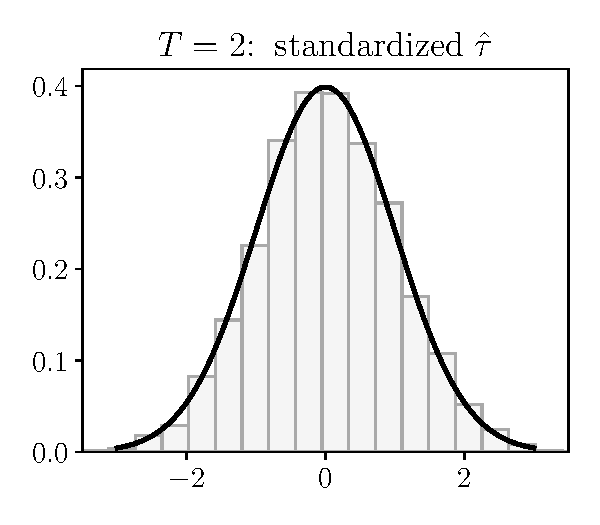
\includegraphics[width=1\linewidth]{plots/simulation/tau_T_2.pdf}
% 		\caption{Flu data}
	\end{subfigure}
	\begin{subfigure}{0.3\textwidth}
		\centering
		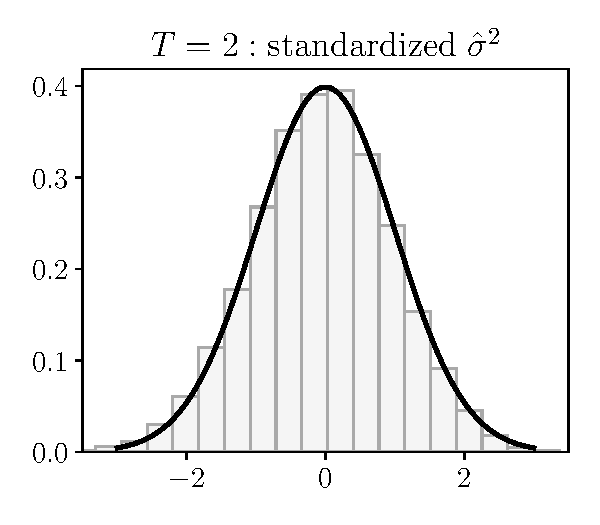
\includegraphics[width=1\linewidth]{plots/simulation/sigma_T_2.pdf}
% 		\caption{Flu data}
	\end{subfigure}
	\begin{subfigure}{0.3\textwidth}
		\centering
		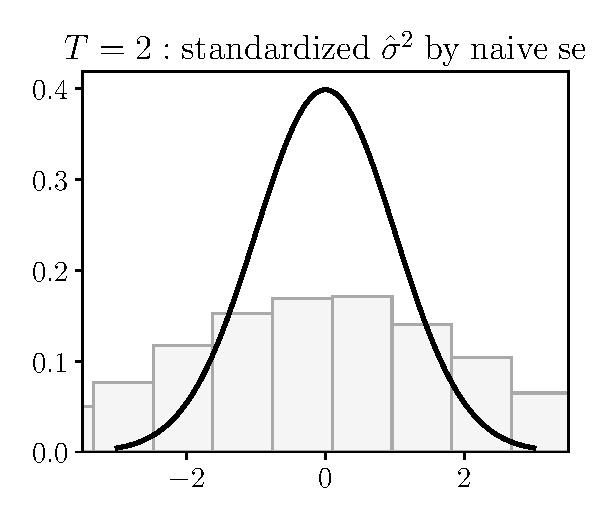
\includegraphics[width=1\linewidth]{plots/simulation/sigma_T_2_wrong.pdf}
% 		\caption{Flu data}
	\end{subfigure}
	\begin{subfigure}{0.3\textwidth}
		\centering
		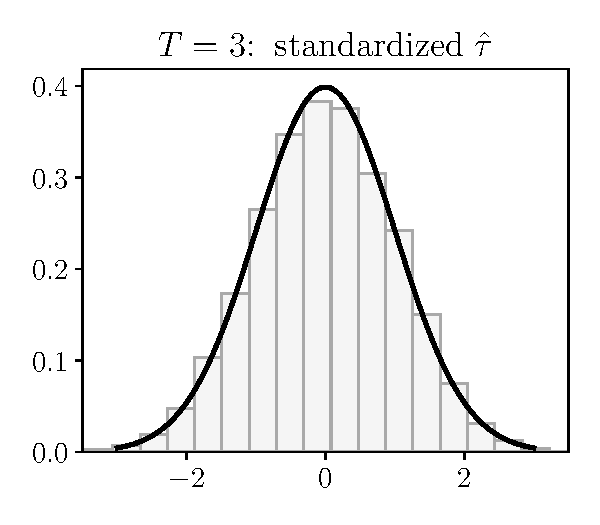
\includegraphics[width=1\linewidth]{plots/simulation/tau_T_3.pdf}
% 		\caption{Flu data}
	\end{subfigure}
	\begin{subfigure}{0.3\textwidth}
		\centering
		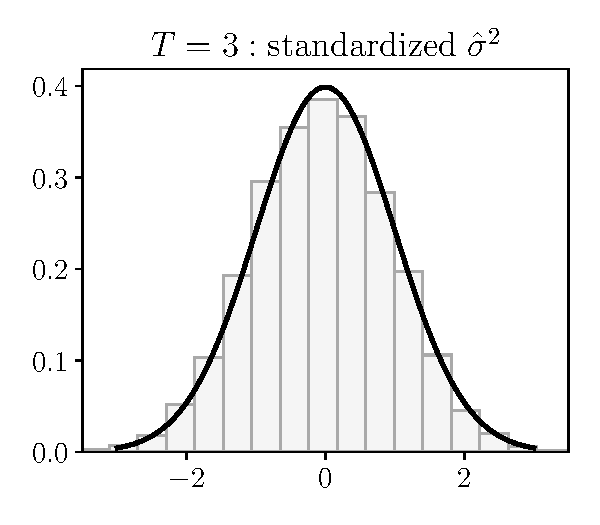
\includegraphics[width=1\linewidth]{plots/simulation/sigma_T_3.pdf}
% 		\caption{Flu data}
	\end{subfigure}
	\begin{subfigure}{0.3\textwidth}
		\centering
		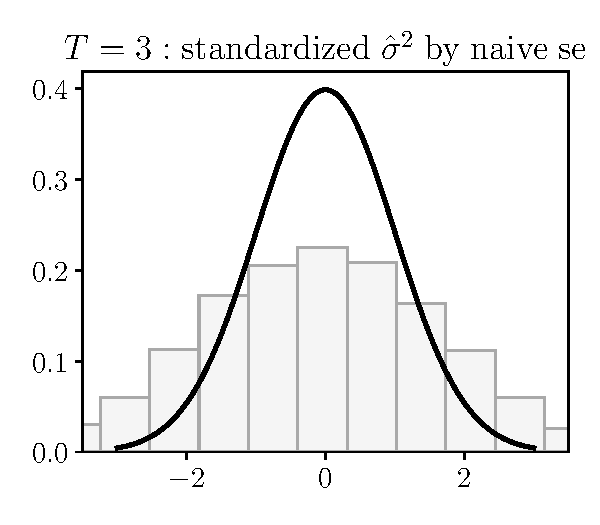
\includegraphics[width=1\linewidth]{plots/simulation/sigma_T_3_wrong.pdf}
% 		\caption{Flu data}
	\end{subfigure}
	\begin{subfigure}{0.3\textwidth}
		\centering
		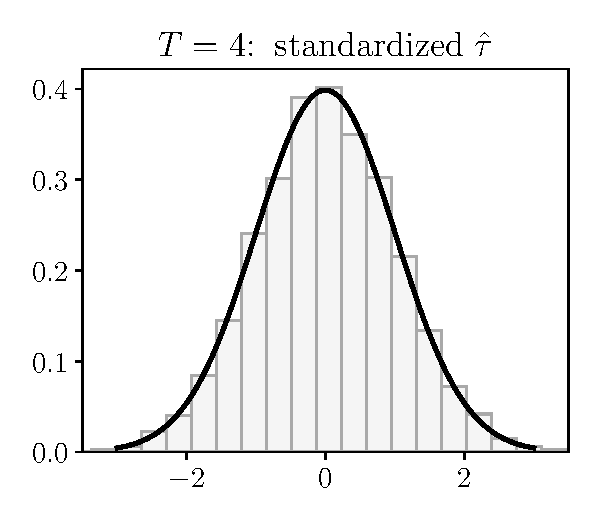
\includegraphics[width=1\linewidth]{plots/simulation/tau_T_4.pdf}
% 		\caption{Flu data}
	\end{subfigure}
	\begin{subfigure}{0.3\textwidth}
		\centering
		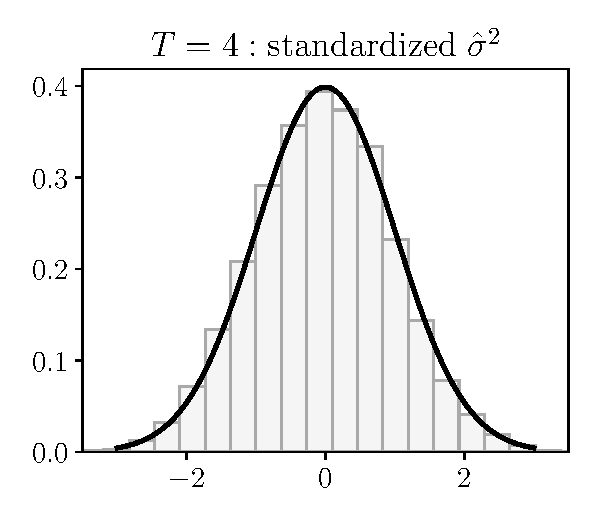
\includegraphics[width=1\linewidth]{plots/simulation/sigma_T_4.pdf}
% 		\caption{Flu data}
	\end{subfigure}
	\begin{subfigure}{0.3\textwidth}
		\centering
		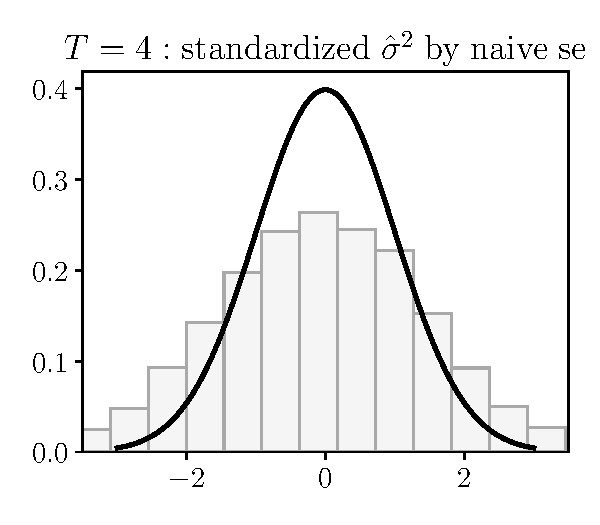
\includegraphics[width=1\linewidth]{plots/simulation/sigma_T_4_wrong.pdf}
% 		\caption{Flu data}
	\end{subfigure}
	\caption{Finite sample properties of Lemma \ref{lemma:asymptotic-tau-sigma}: Histograms of $\hat{\tau}_{\mathsf{ss}}$, $\estsigmasq_{\mathsf{ss}}$, and $\estsigmasq_{{\mathsf{ss}},\mathrm{naive}} $.  The standard normal density function is superimposed on the histograms. $N = 10,000$, $\tau_0 = 3$ and $\sigma=1$.}
	\label{fig:test-asymptotics}
\end{figure}



\begin{table}[h!]
    \centering
\begin{tabular}{l|p{2cm}p{2cm}p{2cm}}
\toprule
  $T$ &  $\widehat{\var}(\hat{\tau}_{\mathsf{ss}})$ &  $\widehat{\var}(\estsigmasq_{\mathsf{ss}})$ &  $\widehat{\mathrm{Cov}}(\hat{\tau}_{\mathsf{ss}}, \estsigmasq_{\mathsf{ss}})$   \\
\midrule
2 & 0.994 & 1.012 & $-0.008$ \\
3 & 1.022 & 1.002 & $-0.008$ \\
4 & 1.005 & 0.994 & 0.001 \\
\bottomrule
\end{tabular}
    \caption{Finite sample properties of Lemma \ref{lemma:asymptotic-tau-sigma}: Estimates of $\var(\hat{\tau}_{\mathsf{ss}})$, $\var(\estsigmasq_{\mathsf{ss}})$, and $\mathrm{Cov}(\hat{\tau}_{\mathsf{ss}}, \estsigmasq_{\mathsf{ss}})$ with $N = 10,000$, $\tau_0 = 3$  and $\sigma=1$. }
    \label{tab:test-asymptotics}
\end{table}

\clearpage

\subsection{Finite Sample Properties of Theorem \ref{theorem:asymptotic-page}}\label{subsec:finite-sample-pgae}

We verify the finite sample properties of Theorem \ref{theorem:asymptotic-page} using simulated data. The data generating process is the same as that in Section \ref{subsec:finite-sample-lemma}. We run adaptive experiments using PGAE that allow for the early termination of the experiment. Let $\tilde{T}$ be the duration of the adaptive experiment.
% Let $T$ be the number of periods that the experiment runs. 

We report the standardized $\hat{\tau}_\all$, that is, 
\[ \hat{\tau}_{\all,{\mathsf{ss}}} =  \sqrt{N} \cdot \frac{\hat{\tau} - \tau_0}{[\estsigmasq_{\ad,2} /(\tilde{T} \cdot \funfrac(\bm{\omega}_{\fcs, 1:\tilde{T}}, \tilde{T}))]^{1/2}}, \]
% and the standardized $\estsigmasq_{\ad,1}$, that is, \[\estsigmasq_{\ad,1,{\mathsf{ss}}} =  \sqrt{N T} \cdot \frac{\estsigmasq_{\ad,1} - \sigma^2}{\hat{\xi}^\dagger_{\ad,1}}, \]
% where $\hat{\xi}_{\ad,1}^\dagger = \sqrt{\estxisq_{\ad,1} + {2}/{(T-1)} \cdot (\estsigmasq_{\ad,1})^2 }$ and $\estxisq_{\ad,1}$ is estimated using the formula \eqref{eqn:fourth-moment-sigma-estimator} on $\mathcal{S}_{\ad,1}$. 
Moreover, we report the standardized $\estsigmasq_{\ad,2}$, that is, \[\estsigmasq_{\ad,2,{\mathsf{ss}}} =  \sqrt{N} \cdot \frac{\estsigmasq_{\ad,2} - \sigma^2}{[\estxidaggersq_{\ad,2}/\tilde{T}]^{1/2} }, \]
where $\estxidaggersq_{\ad,2} = \estxisq_{\ad,2} + {2}/{(\tilde{T}-1)} \cdot (\estsigmasq_{\ad,2})^2$ and $\estxisq_{\ad,2}$ is estimated using the formula \eqref{eqn:fourth-moment-sigma-estimator} on $\mathcal{S}_{\ad,2}$. 

We generate the simulated data and run adaptive experiments for 1,000 times. Note that the experiment termination time varies across the 1,000 iterations, as shown in Figure \ref{fig:experiment-termination-page}. 


We report the histograms of $\hat{\tau}_{\all,s}$ and $\estsigmasq_{\ad,2,{\mathsf{ss}}}$ in Figure \ref{fig:test-asymptotics-page}. The histograms of $\hat{\tau}_{\mathsf{ss}}$ and  $\estsigmasq_{\mathsf{ss}}$ are close to the standard normal density function, showing the good finite sample properties of $\hat{\tau}_{\all,{\mathsf{ss}}}$ and $\estsigmasq_{\ad,2,{\mathsf{ss}}}$ (even though the experiment termination times vary across iterations). 

Furthermore, we report the mean of $\hat{\tau}_{\all,{\mathsf{ss}}}$ and $\estsigmasq_{\ad,2,{\mathsf{ss}}}$, respectively, which serve as the estimates of $\var(\hat{\tau}_{\all,{\mathsf{ss}}})$ and $\var(\estsigmasq_{\ad,2,{\mathsf{ss}}})$ in Table \ref{tab:test-asymptotics}.
They are close to $1$ for various $T_{\max}$, that additionally show the good finite sample properties and verify the asymptotic distribution of $\hat{\tau}_{\all,{\mathsf{ss}}}$ and $\estsigmasq_{\ad,2,{\mathsf{ss}}}$. Moreover, we report the mean of $\hat{\tau}_{\all,{\mathsf{ss}}} \cdot \estsigmasq_{\ad,2,{\mathsf{ss}}}$, which serve as the estimates of $\mathrm{Cov}(\hat{\tau}_{\all,{\mathsf{ss}}}, \estsigmasq_{\ad,2,{\mathsf{ss}}})$, verifying the mutual asymptotic independence between $\hat{\tau}_{\all,{\mathsf{ss}}}$ and $\estsigmasq_{\ad,2,{\mathsf{ss}}}$. 




\begin{figure}[h!]
	\centering
	\begin{subfigure}{0.3\textwidth}
		\centering
		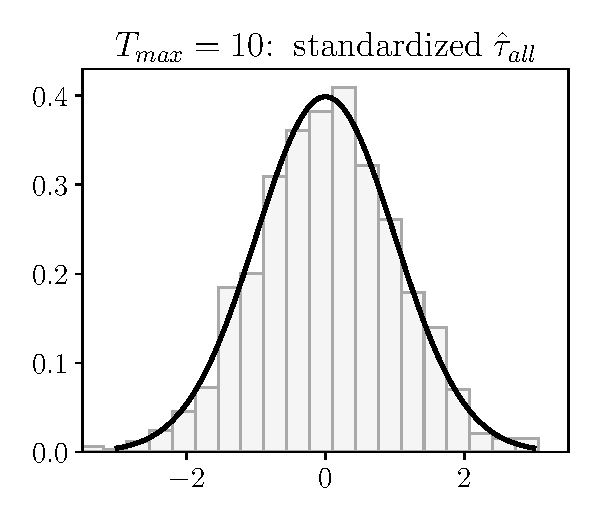
\includegraphics[width=1\linewidth]{plots/simulation/tau_T_10_adaptive.pdf}
	\end{subfigure}%
	\begin{subfigure}{0.3\textwidth}
		\centering
		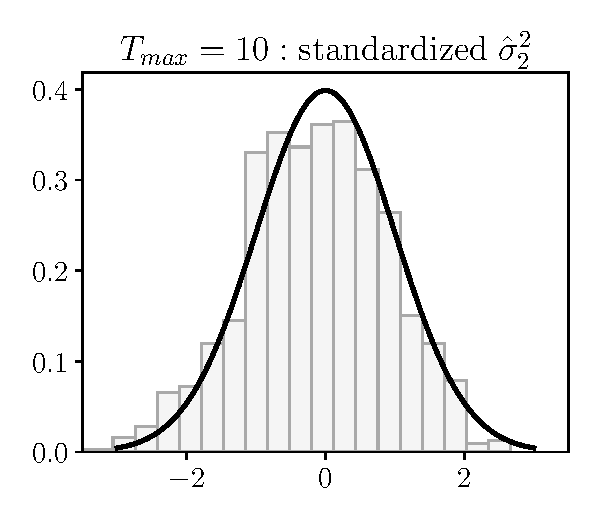
\includegraphics[width=1\linewidth]{plots/simulation/sigma_2_T_10_adaptive.pdf}
	\end{subfigure}
	\begin{subfigure}{0.3\textwidth}
		\centering
		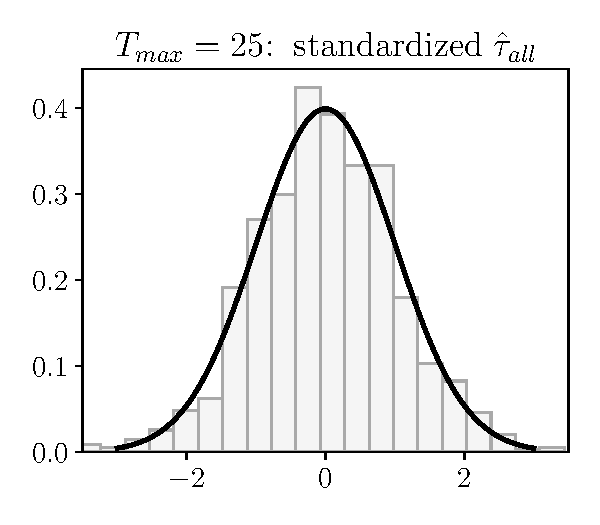
\includegraphics[width=1\linewidth]{plots/simulation/tau_T_25_adaptive.pdf}
	\end{subfigure}%
	% \begin{subfigure}{0.3\textwidth}
	% 	\centering
	% 	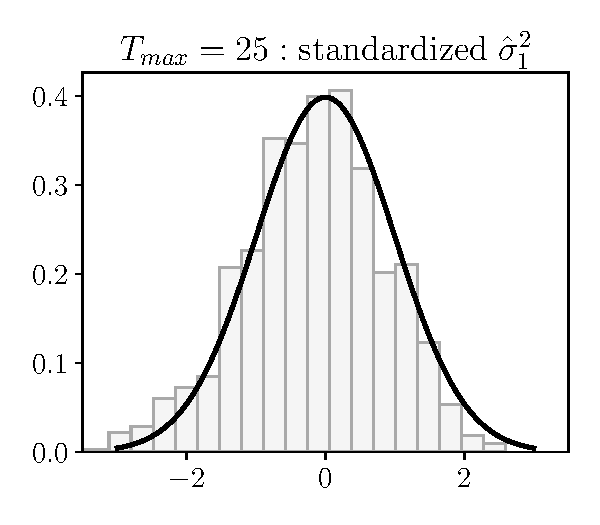
\includegraphics[width=1\linewidth]{plots/simulation/sigma_1_T_25_adaptive.pdf}
	% \end{subfigure}
	\begin{subfigure}{0.3\textwidth}
		\centering
		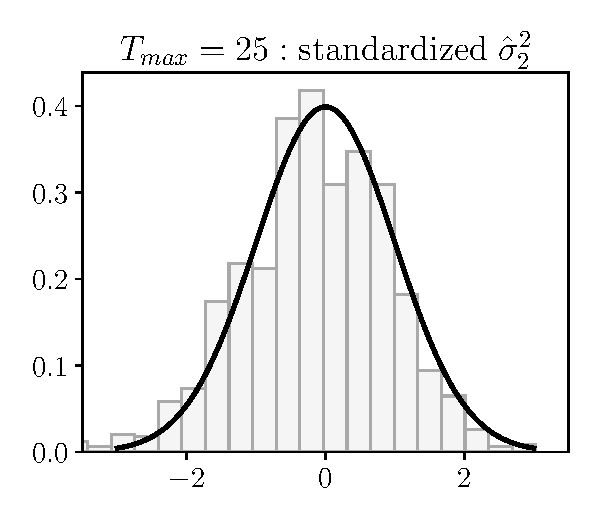
\includegraphics[width=1\linewidth]{plots/simulation/sigma_2_T_25_adaptive.pdf}
	\end{subfigure}
	\caption{Finite sample properties of Theorem  \ref{theorem:asymptotic-page}: Histograms of $\hat{\tau}_{\all,\mathsf{ss}}$ and $\estsigmasq_{\ad,2,\mathsf{ss}}$.  The standard normal density function is superimposed on the histograms. $N = 500$, $\tau_0 = 1$, and $\sigma_\varepsilon=1$}
	\label{fig:test-asymptotics-page}
\end{figure}


\begin{figure}[h!]
	\centering
	\begin{subfigure}{0.25\textwidth}
		\centering
		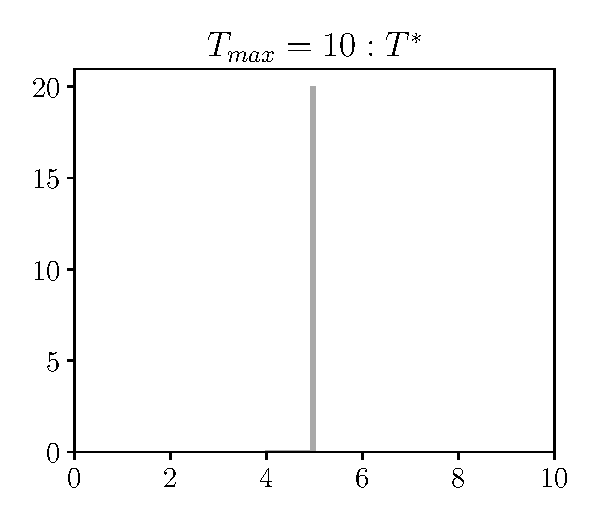
\includegraphics[width=1\linewidth]{plots/simulation/T_10_T_ast_adaptive.pdf}
	\end{subfigure}%
	\begin{subfigure}{0.25\textwidth}
		\centering
		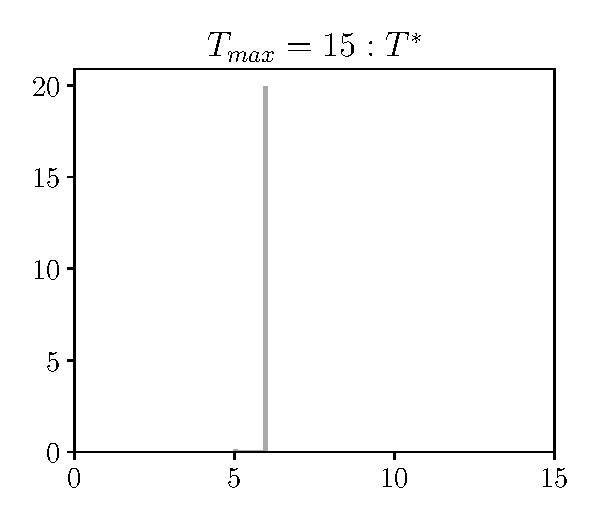
\includegraphics[width=1\linewidth]{plots/simulation/T_15_T_ast_adaptive.pdf}
	\end{subfigure}%
	\begin{subfigure}{0.25\textwidth}
		\centering
		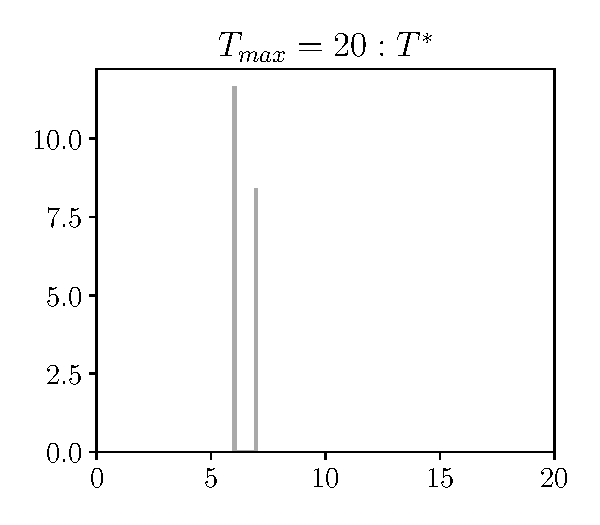
\includegraphics[width=1\linewidth]{plots/simulation/T_20_T_ast_adaptive.pdf}
	\end{subfigure}%
	\begin{subfigure}{0.25\textwidth}
		\centering
		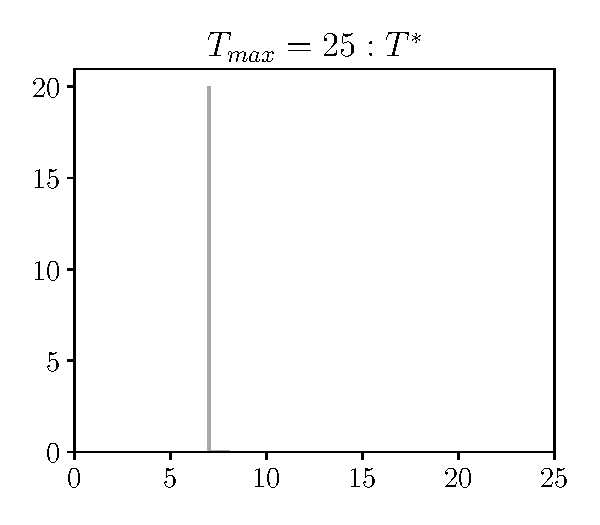
\includegraphics[width=1\linewidth]{plots/simulation/T_25_T_ast_adaptive.pdf}
	\end{subfigure}
	\caption{Histogram of the experiment termination times from PGAE for various $T_{\max}$ with $N = 500$, $\sigma_\varepsilon = 3$ and the threshold for precision $c = N/\sigma_\varepsilon^2 $.}
	\label{fig:experiment-termination-page}
\end{figure}


\begin{table}[h!]
    \centering
% \begin{tabular}{l|p{2.cm}p{2.cm}p{2.cm}p{3cm}p{3cm}p{3.2cm}}
{\footnotesize
\begin{tabular}{l|cccccc}
\toprule
  $T_{\max}$ &  $\widehat{\var}(\hat{\tau}_{\all,{\mathsf{ss}}})$ & $\widehat{\var}(\estsigmasq_{\ad,2,{\mathsf{ss}}})$ & $\widehat{\mathrm{Cov}}(\hat{\tau}_{\all,{\mathsf{ss}}}, \estsigmasq_{\ad,2,{\mathsf{ss}}})$   \\
\midrule
5 &  1.062 &  1.113 &  0.001 \\
10 &  1.013 &  1.076 &  0.006 \\
15 &  1.033 &  1.038 & -0.050 \\
20 &  1.007 &  1.078 & -0.001 \\
25 &  1.035 &  1.113 & -0.016 \\
30 &  1.072 &  1.099 &  0.028 \\
35 &  0.931 &  1.026 & -0.014 \\
\bottomrule
\end{tabular}
}
    \caption{Finite sample properties of Theorem  \ref{theorem:asymptotic-page}: Estimates of $\var(\hat{\tau}_{\all,{\mathsf{ss}}})$, $\var(\estsigmasq_{\ad,2,{\mathsf{ss}}})$, and $\Cov(\hat{\tau}_{\all,{\mathsf{ss}}}, \estsigmasq_{\ad,2,{\mathsf{ss}}})$ with $N = 500$, $\tau_0 = 1$, $\sigma_\varepsilon=1$.}
    \label{tab:theorem-asymptotic-covariance}
\end{table}